
\documentclass[11pt]{article}
 
\usepackage[margin=1in]{geometry} 
\usepackage{amsmath,amsthm,amssymb,scrextend}
\usepackage{fancyhdr}
\pagestyle{fancy}

\newcommand{\cont}{\subseteq}
\usepackage{csvsimple}
\usepackage{tikz}
\usepackage{pgfplots}
\usepackage{amsmath}
\usepackage[mathscr]{euscript}
\let\euscr\mathscr \let\mathscr\relax% just so we can load this and rsfs
\usepackage[scr]{rsfso}
\usepackage{amsthm}
\usepackage{amssymb}
\usepackage{multicol}
\usepackage[colorlinks=true, pdfstartview=FitV, linkcolor=blue,
citecolor=blue, urlcolor=blue]{hyperref}

\usepackage{setspace}
\onehalfspacing

\usepackage{siunitx} % 用于处理数字和单位


\DeclareMathOperator{\arcsec}{arcsec}
\DeclareMathOperator{\arccot}{arccot}
\DeclareMathOperator{\arccsc}{arccsc}
\newcommand{\ddx}{\frac{d}{dx}}
\newcommand{\dfdx}{\frac{df}{dx}}
\newcommand{\ddxp}[1]{\frac{d}{dx}\left( #1 \right)}
\newcommand{\dydx}{\frac{dy}{dx}}
\let\ds\displaystyle
\newcommand{\intx}[1]{\int #1 \, dx}
\newcommand{\intt}[1]{\int #1 \, dt}
\newcommand{\defint}[3]{\int_{#1}^{#2} #3 \, dx}
\newcommand{\imp}{\Rightarrow}
\newcommand{\un}{\cup}
\newcommand{\inter}{\cap}
\newcommand{\ps}{\mathscr{P}}
\newcommand{\set}[1]{\left\{ #1 \right\}}
\newtheorem*{sol}{Solution}
\newtheorem*{claim}{Claim}

\newcounter{question}
\newenvironment{Question}{%
    \stepcounter{question}%
    \textbf{Question (\alph{question})}%
}{}

\begin{document}
 
% EVERYTHING ABOVE THIS LINE IS JUST PREABLE, NO NEED TO MESS WITH IT.__________________________________________________________________________________________
%

\lhead{FIN3080 Assignment 1}
\chead{LIU, Junle \ 122090337}
\rhead{\today}

% \maketitle
\begin{spacing}{1.5}

\section*{Problem 1}

\noindent
\textbf{Overview}

The overall steps are given in the homework instruction. In this report I will discuss about some detailed manipulations and show the study results.

\noindent
\textbf{Data Collection}

The data are all downloaded from CSMAR as required by the problem, namely the Daily Market Returns, Daily Stock Price Returns, Index per Share, Statements Release Dates over 2016 to 2022 (some data in 2014 and 2015 are included for window operations).



\noindent
\textbf{Step 1 \& 2} 

The data is downloaded and read as DataFrame as required. Noted that there are so many files if we choose .csv files. `.concat' function can easily combine these files together in y axis. The columns are renamed accordingly as well.


\noindent
\textbf{Step 3} 

The EPS file is read and converted to DataFrame. Because excluding parent statements is required, all the rows with `statement\_type' are deleted.

\begin{claimbox}
  On step 3.3, the instruction requires to delete stock names starting with ST and PT. However, some stocks names may coincidentally start with PT/ST (e.g. 836871.BJ PTE). Therefore, I use the Chinese version of stock names, and deleted all stocks starting with ST, PT, *ST, SST, S*ST (once they have such prefix in one period, I delete the company completely).
\end{claimbox}

Then step 3.4 -- 3.6 are some time manipulation procedure, with the usage of pd.to\_datetime \& to\_period. 

\begin{warningbox}
  On step 3.7 \& 3.8, we can NOT directly use `.shift()', because there exists cases that the downloaded data only include December EPS at some random years. So the data can be completely messy if using `.groupby()' + `.shift()' or `.diff()'.
\end{warningbox}

Thus, step 3.7 \& 3.8 are rather complex. I first extract EPS values for June and December in the same year, then calculates the difference between December EPS and June EPS, reflecting the EPS change for the second half of the fiscal year. This result replaces the original December EPS in the data. Noted that the code processes this calculation by grouping the data by stock code and applying these functions to each group, updating the entire dataset accordingly.

Continue on step 3.9, now `.shift()' can be used, because step 3.8 ensures that the data is well structured (all the years with only one entry data will be discarded because of `.dropna()')

Steps3.11 -- 3.13 are steps for correctly derive the SUE deciles. Noted that `.pivot()' is used for converting the long DataFrame to wide DataFrame.

\begin{claimbox}
  On Step 3.9, UE's from the subtraction of this year’s EPS with last year’s. As 2014h1 \& 2014h2 do not have ``last year” in the data set, so their UE will be NaN. On Step 3.10, we include the recent three periods’ data as the window for s.d. Thus, 2015h1, 2015h2 and 2016h1 will be used to get s.d. for 2016h2, and these three periods will not have their own SUE, instead they are NaN and be discarded. That's why the wide data set of EPS from Step 3.13 may start with 2016h2 instead of 2016h1.
\end{claimbox}


\noindent
\textbf{Step 4} 

Very similar to the process to get wide DataFrame in step 3.13, with an additional step to convert the body data into datetime. 


\noindent
\textbf{Step 5} 

All the useful DataFrame we got above are combined into a wide one using `pd.merge()'.


\noindent
\textbf{Step 6} 

Step 6.3 is complex. It uses a loop for iterating on every time period column. The implementation follows the method 2 to get event day in the tutorial slide. For each iteration, the NaN data will be discarded, then the cumulative return of each decile is calculated using `.cumsum()'.

\begin{warningbox}
  Directly using the method on tutorial may cause some time disruption due to unexpected trading suspension (without PT/ST labeled, e.g 000716.SZ). Thus, I limited the original trading date range before getting the relative trading date difference. Data out of range will be discarded for data accuracy.
\end{warningbox}

On step 6.4, we get the mean of decile cumulative return of all half-year periods, namely `mean\_portfolio\_car'. Finally we can get the result figure of this event study:


\begin{figure}[ht]
\centering
% \vspace{-0.43cm}
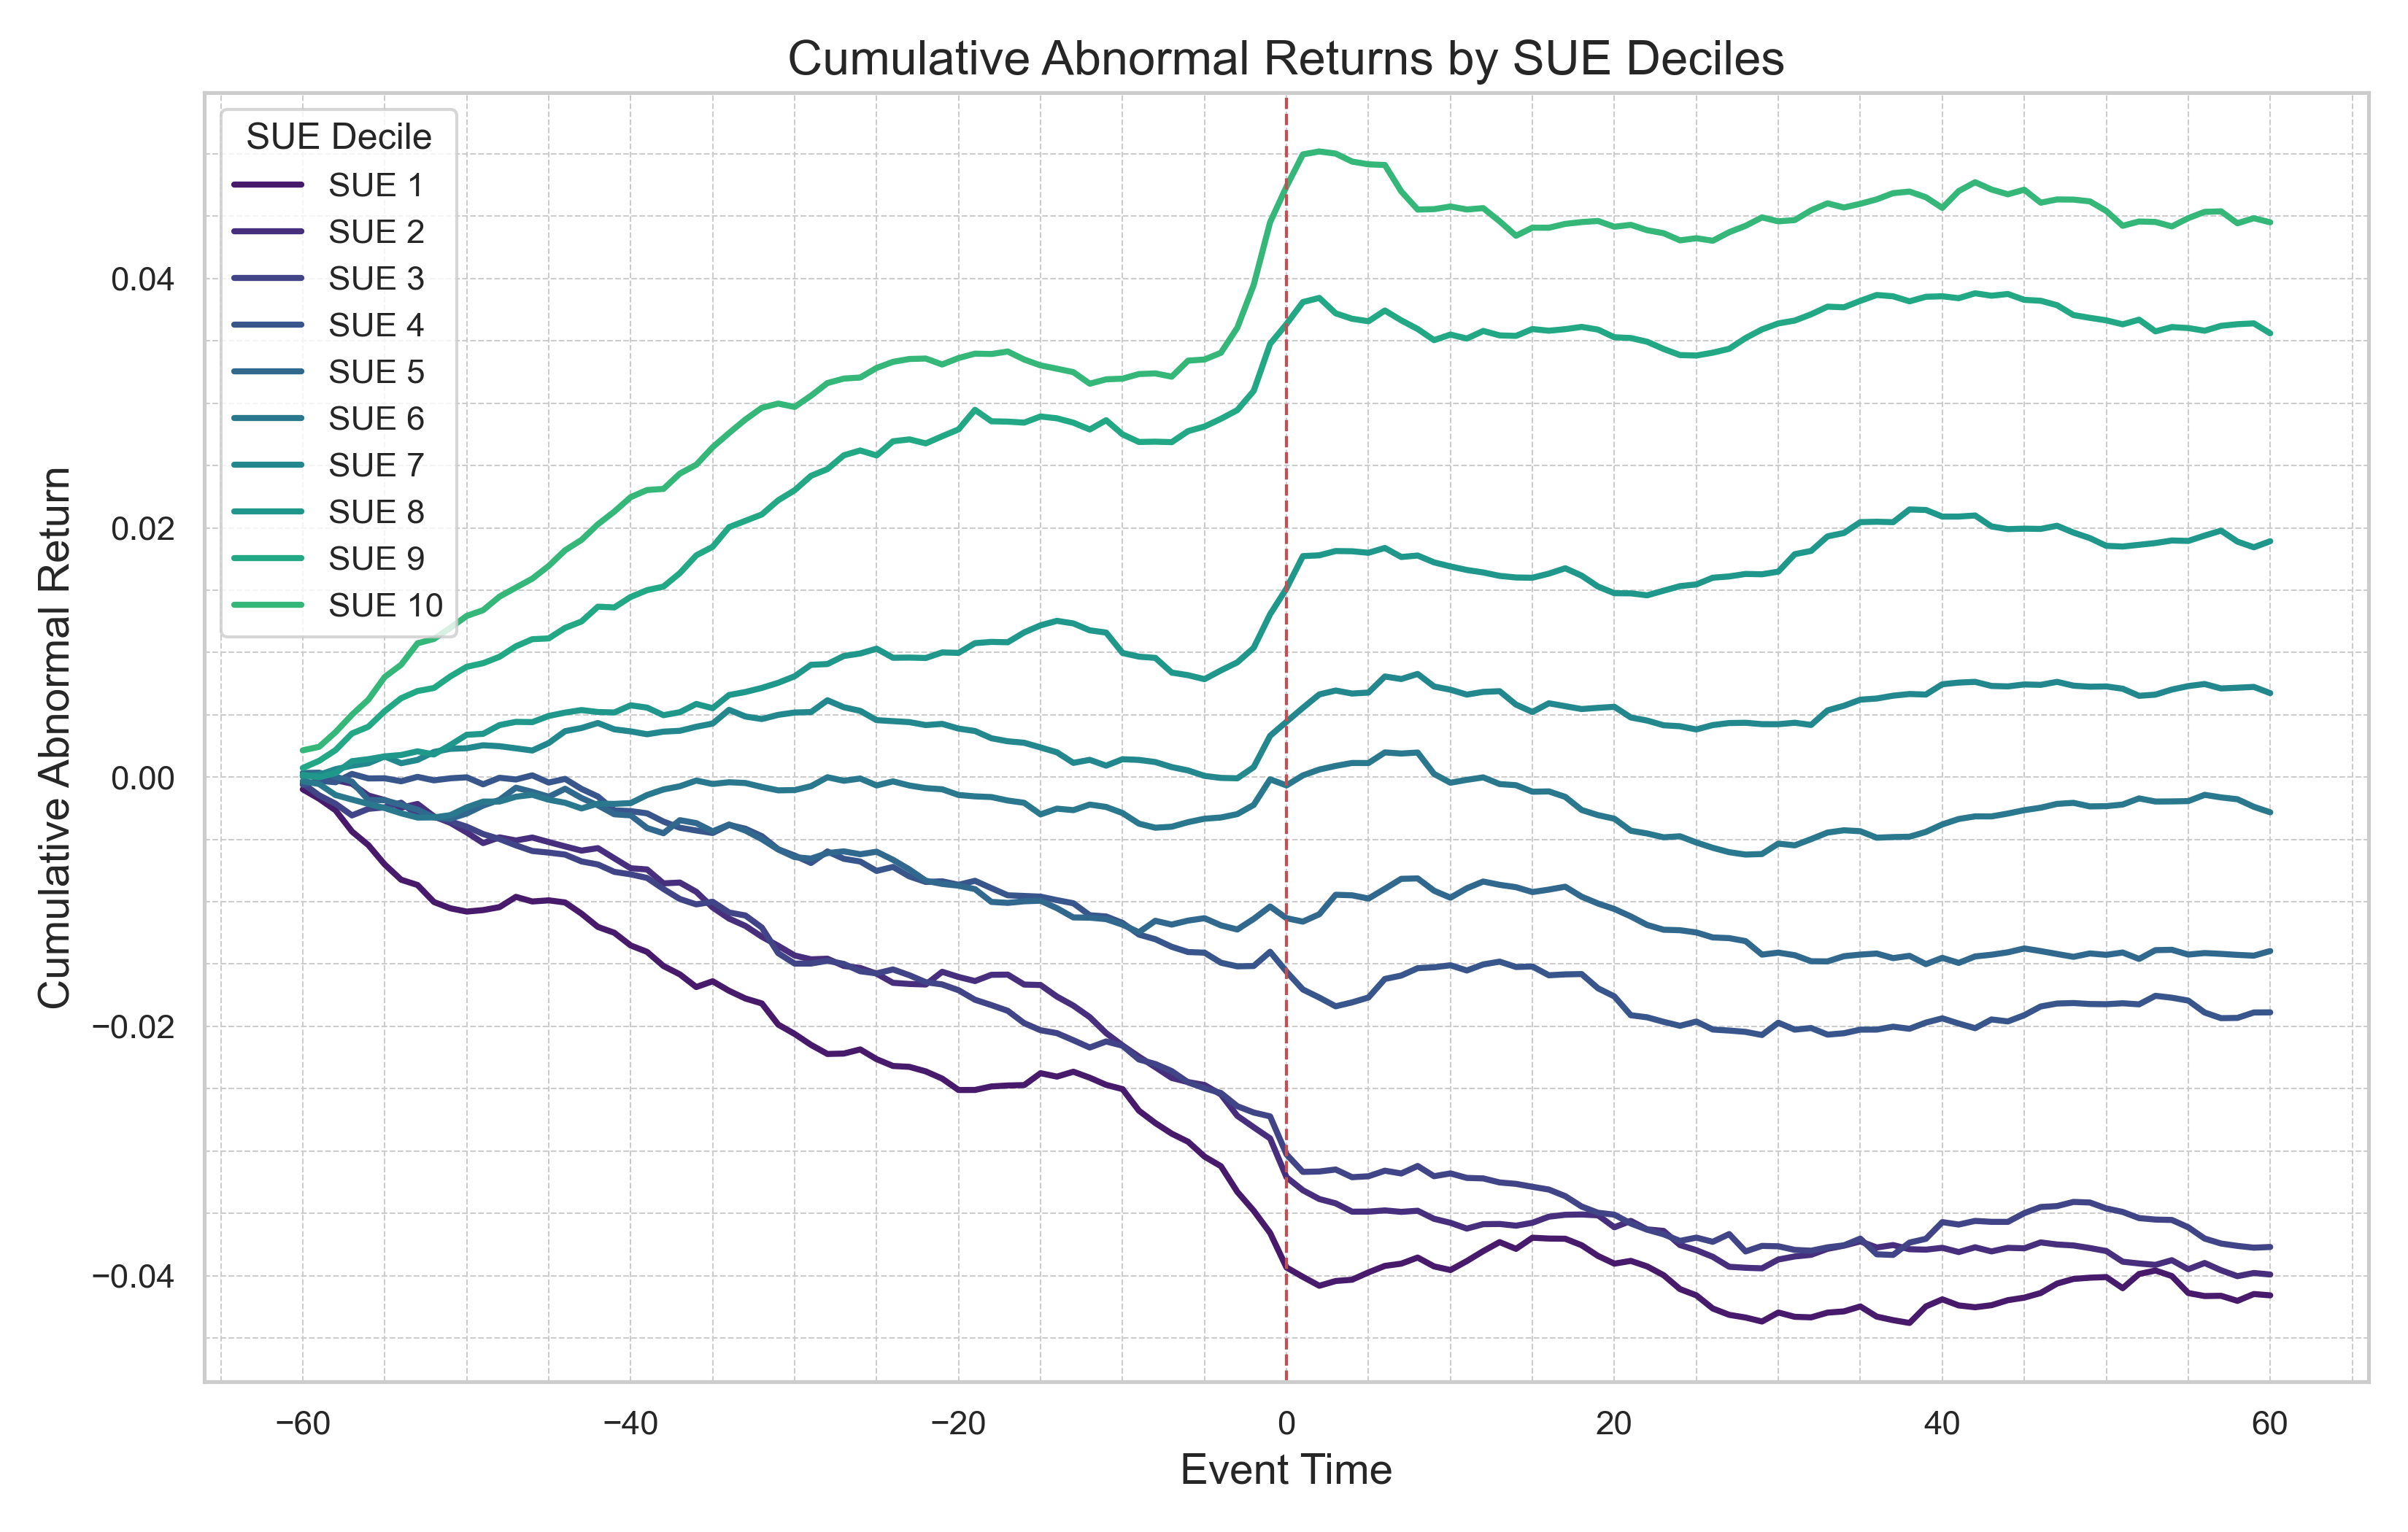
\includegraphics[width=1\textwidth]{data/Result Figure.png}
\caption{Cumulative Abnormal Returns by SUE Deciles}
\label{fig:example}
\end{figure}


\noindent
\textbf{Results}

As shown in the figure, the diciles with higher SUE (SUE 6 -- 10) has higher cumulative abnormal returns with increasing trends; the diciles with lower SUE (SUE 1 -- 4) has lower (more negative) cumulative abnormal returns with decreasing trends.

In conclusion, Post Earnings Announcement Drift (PEAD) exists in China’s A-share markets.


\vspace{1.5cm}

\centering -- END --

\section*{Problem 2}

\noindent
\textbf{Data Collection}

The data are all downloaded from CSMAR as required, namely Returns Without Cash Dividend Reinvested from 2017-01 to 2022-53 (YYYY-WW).

As required, the time period should be divided to three parts. In this question, 2 years will be one regression period, namely 2017-2018 (first regression), 2019-2020 (second regression), 2021-2022 (third regression).

\\

\noindent
\textbf{Steps}

(a) \textit{Data Manipulation.} We can simply use $.concat()$ to connect the two .csv files downloaded. Besides, I take out market type 1, 4, 64, which are the codes for A-share mainboard as required.

(b) \textit{Market Return.} Use $.groupby(`week')$ and $.mean()$ to calculate the market return by covering all stock returns.

(c) \textit{Data Manipulation.} Just load the data, and align the `week' data type and structure using some string methods.

(d) \textit{Process.} 

\noindent
\textbf{Replicate Table 2 from the referenced paper.}

Firstly, regress every stock return on the market return, so we can get the beta in single factor models in the first time period. Then, after sorting and ranking beta, we divide the stocks into 10 groups. We construct 10 portfolios by combining all the stocks in each group. Then we calculate the difference among return and risk-free rate. Finally we can get regression result in Table 2 using the second period data.

\begin{table}[htbp]
    \centering
    \caption{\textbf{(Table 2 in paper)} Time series regression results of the second period of portfolio}
    \vspace{0.4cm}
    \csvautotabular{data/Table_2_result.csv}
\end{table}

Note: all the data are round to five decimals.

\noindent
\textbf{Results.} By comparing with the paper given, we find the results are a little different:

1. The Beta values across all portfolios are fairly consistent, typically  around 1. Moreover, the p values are consistently low, showing the significant impact of market returns on stock returns. This aligns with the findings of the referenced paper.

2. Initially, the R-squared values are consistently high, indicating that our regression model effectively captures the variance in stock returns. Furthermore, there's no notable increase in R-squared values with higher Beta values, implying that factors beyond systematic risk influence stock returns. This aligns with the referenced paper.

3. However, the alpha values we computed are notably small, approaching zero. Based on the t value and p value, we lack sufficient evidence to reject the null hypothesis that alpha equals zero. This does NOT align with the referenced paper.


\noindent
\textbf{Replicate Table 3 from the referenced paper.}

I firstly take out the third period data from 2021-2022. Then calculate the average excess return, and merge corresponding beta to the dataframe. By repeating the regression in the paper, we can get:

\begin{table}[htbp]
    \centering
    \caption{\textbf{(Table 3 in paper)} Cross-sectional regression results of the third period of portfolio}
    \vspace{0.4cm}
    \csvautotabular{data/Table_3_result.csv}
\end{table}

Note: all the data are round to five decimals.


\noindent
\textbf{Results.} Based on the table above, the following conclusions can be drawn:

1. The R-squared value stands at only 0.45885, similar to the explaining power in the paper.

2. The value of gamma1 is 0.00266, and t-statistics is greater than 2, p-value is 0.031 (smaller than 0.05) as well, showing statistically significant positive correlation between returns and systematic risk. This suggests that returns tend to rise with increasing systematic risk, consistent with the principles of the CAPM model, and aligns with the conclusions drawn in the reference paper.

3. However, the alpha values obtained are notably small, approaching zero. The t-value is rather close to 0 (greater than -2), p-value is 0.324, so we fail to find sufficient evidence to reject the null hypothesis that alpha equals zero. This contradicts the assertions in the reference paper. 

Possible reason:
Chinese stock market has undergone rapid development in these years after the paper published, becoming substantially more efficient over time. The establishment and enhancement of the multi-level market system, alongside reforms in the new stock issuance system, have contributed to the maturation of China's securities market. Consequently, the equilibrium relationship between risk and return in securities investment is increasingly manifested, leading to a diminishing impact of non-systematic risks on pricing. As a result, alpha is not significantly different from zero.








\section*{Problem 3}

\textit{Table.} From 2011 to 2020. All numbers are roud to four decimals.


\begin{table}[htbp]
    \centering
    \caption{The Annual Median for ROE and Total Revenue Growth Rate}
    \vspace{0.4cm}
    \csvautotabular{data/AS_1_p3_median.csv}
\end{table}

\ 


\textit{Graph.} From 2011 to 2020.

\begin{figure}[h]
\centering
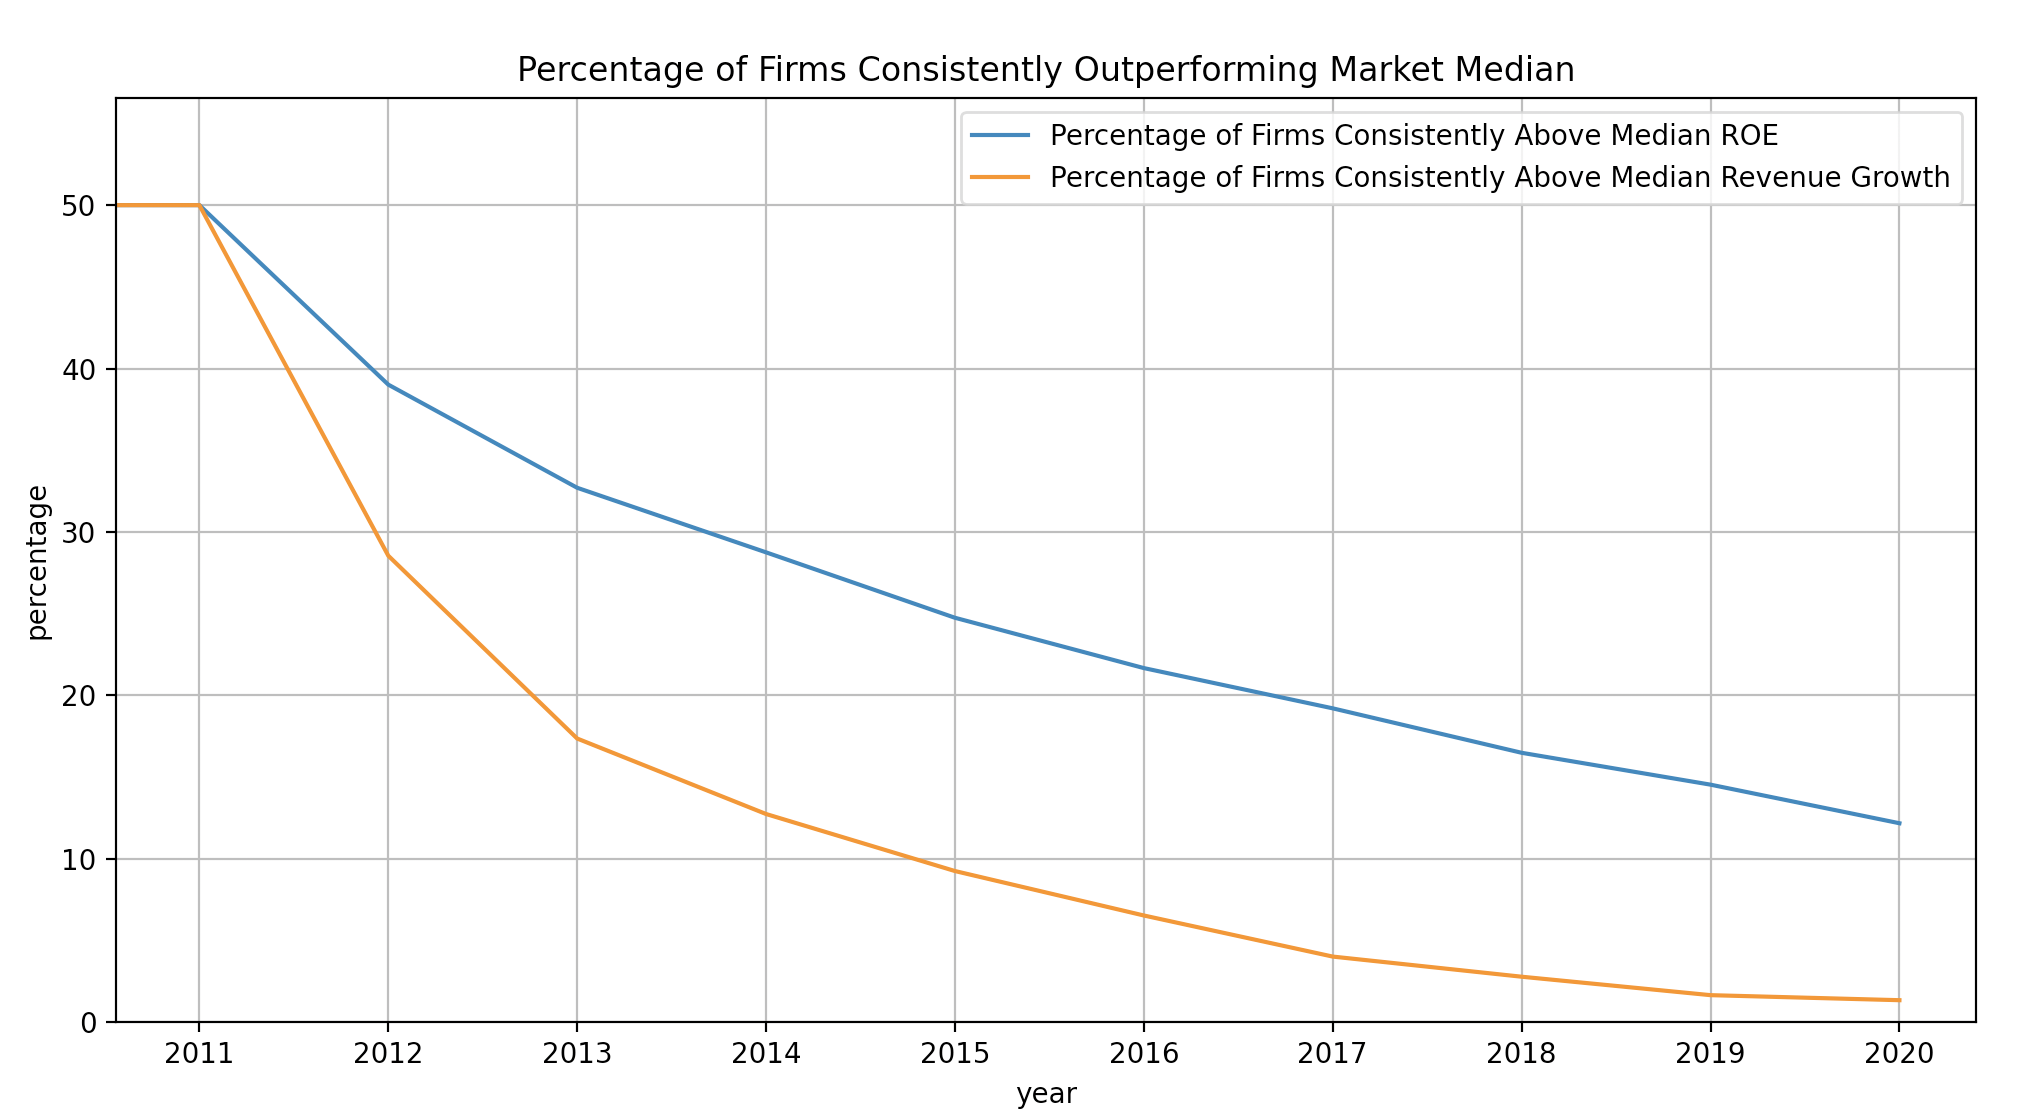
\includegraphics[width=1\textwidth]{data/pct_consistent_outperformer.png}
\caption{Time-series of the percentages of companies that consistently maintain above-median ROE and total revenue growth rate}
\label{fig:example}
\end{figure}

Noted that it represents the percentage of firms that outperform consistently than the median ROE and revenue growth rate, repectively.

\end{spacing}

 


% THE DOCUMENT IS ESSENTIALLY DONE AT THIS POINT, NO NEED TO EDIT ANYTHING BELOW THIS______________________________________________________________________________________________

\end{document}